%% FEUP THESIS STYLE for LaTeX2e
%% how to use feupteses for MIEIC dissertations
%%
%% FEUP, JCL & JCF,  Wed Oct  4 16:32:24 2017
%%
%% PLEASE send improvements to jlopes at fe.up.pt and to jcf at fe.up.pt
%%

%%========================================
%% Commands: pdflatex thesis
%%           bibtex thesis
%%           makeindex thesis (only if creating an index) 
%%           pdflatex thesis
%% Alternative:
%%          latexmk -pdf thesis.tex
%%========================================

\documentclass[11pt,a4paper,twoside,openright]{report}
\usepackage[utf8]{inputenc}
%\usepackage[latin1]{inputenc}

%%%%%%% English version 

%% MIEIC options
\usepackage[mieic]{feupteses}                  % work version
%\usepackage[mieic,juri]{feupteses}             % juri verrion
%\usepackage[mieic,final]{feupteses}            % final version

%% Additional options for feupteses.sty: 
%% - portugues: titles, etc in portuguese
%% - onpaper: links are not shown (for paper versions)
%% - backrefs: include back references from bibliography to citation place

%%%%%%% Portuguese version

%\usepackage[mieic,portugues]{feupteses}        % work version
%\usepackage[mieic,portugues,juri]{feupteses}   % juri version
%\usepackage[mieic,portugues,final]{feupteses}  % final version

%% Uncomment the next lines if side by side graphics used
%\usepackage[lofdepth,lotdepth]{subfig}
%\usepackage{graphicx}
%\usepackage{float}

%% Include color package
\usepackage{hyperref,xcolor}
\definecolor{cloudwhite}{cmyk}{0,0,0,0.025}
\definecolor{engineering}{rgb}{0.549, 0.176, 0.098}
\hypersetup {
    colorlinks=true,
    linkcolor=engineering,
    urlcolor={engineering},
    filecolor={engineering},
    citecolor={engineering},
    allcolors={engineering}
}

%% Include source-code listings package
\usepackage{listings}
\lstset{ %
 language=C,                        % choose the language of the code
 basicstyle=\footnotesize\ttfamily,
 keywordstyle=\bfseries,
 numbers=left,                      % where to put the line-numbers
 numberstyle=\scriptsize\texttt,    % the size of the fonts that are used for the line-numbers
 stepnumber=1,                      % the step between two line-numbers. If it's 1 each line will be numbered
 numbersep=8pt,                     % how far the line-numbers are from the code
 frame=tb,
 float=htb,
 aboveskip=8mm,
 belowskip=4mm,
 backgroundcolor=\color{cloudwhite},
 showspaces=false,                  % show spaces adding particular underscores
 showstringspaces=false,            % underline spaces within strings
 showtabs=false,                    % show tabs within strings adding particular underscores
 tabsize=2,	                    % sets default tabsize to 2 spaces
 captionpos=b,                      % sets the caption-position to bottom
 breaklines=true,                   % sets automatic line breaking
 breakatwhitespace=false,           % sets if automatic breaks should only happen at whitespace
 escapeinside={\%*}{*)},            % if you want to add a comment within your code
 morekeywords={*,var,template,new}  % if you want to add more keywords to the set
}

%% Allow for better aligning of equations
\usepackage{amsmath}

\usepackage{dirtytalk}
%% Uncomment to create an index (at the end of the document)
%\makeindex

%% Path to the figures directory
%% TIP: use folder ``figures'' to keep all your figures
\graphicspath{{figures/}}

%%----------------------------------------
%% TIP: if you want to define more macros, use an external file to keep them
%some macro definitions

% format
\newcommand{\class}[1]{{\normalfont\slshape #1\/}}

% entities
\newcommand{\Feup}{Faculdade de Engenharia da Universidade do Porto}

\newcommand{\svg}{\class{SVG}}
\newcommand{\scada}{\class{SCADA}}
\newcommand{\scadadms}{\class{SCADA/DMS}}

%%----------------------------------------

%%========================================
%% Start of document
%%========================================
\begin{document}

%%----------------------------------------
%% Information about the work
%%----------------------------------------
\title{Title of the Dissertation}
\author{Name of the Author}

%% Uncomment next line for date of submission
%\thesisdate{July 31, 2008}

%%Uncomment next line for copyright text if used
%\copyrightnotice{Name of the Author, 2008}

\supervisor{Supervisor}{Name of the Supervisor}

%% Uncomment next line if necessary
%\supervisor{Second Supervisor}{Name of the Supervisor}

%% Uncomment committee stuff in the final version 
%\committeetext{Approved in oral examination by the committee:}
%\committeemember{Chair}{Prof.\ Name of the President}
%\committeemember{External Examiner}{Prof.\  Name of the Examiner}
%\committeemember{Supervisor}{Prof.\ Name of the Supervisor}

%\committeetext{Aprovado em provas públicas pelo Júri:}
%\committeemember{Presidente}{Prof.\ Nome do presidente do júri}
%\committeemember{Arguente}{Prof.\ Nome do arguente do júri}
%\committeemember{Vogal}{Prof.\ Nome do vogal do júri}

%% Specify cover logo (in folder ``figures'')
\logo{uporto-feup.pdf}

%% Uncomment next line for additional text below the author's name (front page)
%\additionalfronttext{Preparação da Dissertação}

%%----------------------------------------
%% Preliminary materials
%%----------------------------------------

% remove unnecssary \include{} commands
\begin{Prolog}
  \chapter*{Abstract}

Lorem ipsum dolor sit amet, consectetuer adipiscing elit. Sed vehicula
lorem commodo dui. Fusce mollis feugiat elit. Cum sociis natoque
penatibus et magnis dis parturient montes, nascetur ridiculus
mus. Donec eu quam. Aenean consectetuer odio quis nisi. Fusce molestie
metus sed neque. Praesent nulla. Donec quis urna. Pellentesque
hendrerit vulputate nunc. Donec id eros et leo ullamcorper
placerat. Curabitur aliquam tellus et diam. 

Ut tortor. Morbi eget elit. Maecenas nec risus. Sed ultricies. Sed
scelerisque libero faucibus sem. Nullam molestie leo quis
tellus. Donec ipsum. Nulla lobortis purus pharetra turpis. Nulla
laoreet, arcu nec hendrerit vulputate, tortor elit eleifend turpis, et
aliquam leo metus in dolor. Praesent sed nulla. Mauris ac augue. Cras
ac orci. Etiam sed urna eget nulla sodales venenatis. Donec faucibus
ante eget dui. Nam magna. Suspendisse sollicitudin est et mi. 

Fusce sed ipsum vel velit imperdiet dictum. Sed nisi purus, dapibus
ut, iaculis ac, placerat id, purus. Integer aliquet elementum
libero. Phasellus facilisis leo eget elit. Nullam nisi magna, ornare
at, aliquet et, porta id, odio. Sed volutpat tellus consectetuer
ligula. Phasellus turpis augue, malesuada et, placerat fringilla,
ornare nec, eros. Class aptent taciti sociosqu ad litora torquent per
conubia nostra, per inceptos himenaeos. Vivamus ornare quam nec sem
mattis vulputate. Nullam porta, diam nec porta mollis, orci leo
condimentum sapien, quis venenatis mi dolor a metus. Nullam
mollis. Aenean metus massa, pellentesque sit amet, sagittis eget,
tincidunt in, arcu. Vestibulum porta laoreet tortor. Nullam mollis
elit nec justo. In nulla ligula, pellentesque sit amet, consequat sed,
faucibus id, velit. Fusce purus. Quisque sagittis urna at quam. Ut eu
lacus. Maecenas tortor nibh, ultricies nec, vestibulum varius, egestas
id, sapien. 

Phasellus ullamcorper justo id risus. Nunc in leo. Mauris auctor
lectus vitae est lacinia egestas. Nulla faucibus erat sit amet lectus
varius semper. Praesent ultrices vehicula orci. Nam at metus. Aenean
eget lorem nec purus feugiat molestie. Phasellus fringilla nulla ac
risus. Aliquam elementum aliquam velit. Aenean nunc odio, lobortis id,
dictum et, rutrum ac, ipsum. 

Ut tortor. Morbi eget elit. Maecenas nec risus. Sed ultricies. Sed
scelerisque libero faucibus sem. Nullam molestie leo quis
tellus. Donec ipsum. Nulla lobortis purus pharetra turpis. Nulla
laoreet, arcu nec hendrerit vulputate, tortor elit eleifend turpis, et
aliquam leo metus in dolor. Praesent sed nulla. Mauris ac augue. Cras
ac orci. Etiam sed urna eget nulla sodales venenatis. Donec faucibus
ante eget dui. Nam magna. Suspendisse sollicitudin est et mi. 

Phasellus ullamcorper justo id risus. Nunc in leo. Mauris auctor
lectus vitae est lacinia egestas. Nulla faucibus erat sit amet lectus
varius semper. Praesent ultrices vehicula orci. 

Ut tortor. Morbi eget elit. Maecenas nec risus. Sed ultricies. Sed
scelerisque libero faucibus sem. Nullam molestie leo quis
tellus. Donec ipsum. 

\vspace*{10mm}\noindent
\textbf{Keywords}: keyword1, Keyword2, keyword3

\chapter*{Resumo}

Lorem ipsum dolor sit amet, consectetuer adipiscing elit. Sed vehicula
lorem commodo dui. Fusce mollis feugiat elit. Cum sociis natoque
penatibus et magnis dis parturient montes, nascetur ridiculus
mus. Donec eu quam. Aenean consectetuer odio quis nisi. Fusce molestie
metus sed neque. Praesent nulla. Donec quis urna. Pellentesque
hendrerit vulputate nunc. Donec id eros et leo ullamcorper
placerat. Curabitur aliquam tellus et diam. 

Ut tortor. Morbi eget elit. Maecenas nec risus. Sed ultricies. Sed
scelerisque libero faucibus sem. Nullam molestie leo quis
tellus. Donec ipsum. Nulla lobortis purus pharetra turpis. Nulla
laoreet, arcu nec hendrerit vulputate, tortor elit eleifend turpis, et
aliquam leo metus in dolor. Praesent sed nulla. Mauris ac augue. Cras
ac orci. Etiam sed urna eget nulla sodales venenatis. Donec faucibus
ante eget dui. Nam magna. Suspendisse sollicitudin est et mi. 

Fusce sed ipsum vel velit imperdiet dictum. Sed nisi purus, dapibus
ut, iaculis ac, placerat id, purus. Integer aliquet elementum
libero. Phasellus facilisis leo eget elit. Nullam nisi magna, ornare
at, aliquet et, porta id, odio. Sed volutpat tellus consectetuer
ligula. Phasellus turpis augue, malesuada et, placerat fringilla,
ornare nec, eros. Class aptent taciti sociosqu ad litora torquent per
conubia nostra, per inceptos himenaeos. Vivamus ornare quam nec sem
mattis vulputate. Nullam porta, diam nec porta mollis, orci leo
condimentum sapien, quis venenatis mi dolor a metus. Nullam
mollis. Aenean metus massa, pellentesque sit amet, sagittis eget,
tincidunt in, arcu. Vestibulum porta laoreet tortor. Nullam mollis
elit nec justo. In nulla ligula, pellentesque sit amet, consequat sed,
faucibus id, velit. Fusce purus. Quisque sagittis urna at quam. Ut eu
lacus. Maecenas tortor nibh, ultricies nec, vestibulum varius, egestas
id, sapien. 

Phasellus ullamcorper justo id risus. Nunc in leo. Mauris auctor
lectus vitae est lacinia egestas. Nulla faucibus erat sit amet lectus
varius semper. Praesent ultrices vehicula orci. Nam at metus. Aenean
eget lorem nec purus feugiat molestie. Phasellus fringilla nulla ac
risus. Aliquam elementum aliquam velit. Aenean nunc odio, lobortis id,
dictum et, rutrum ac, ipsum. 

Ut tortor. Morbi eget elit. Maecenas nec risus. Sed ultricies. Sed
scelerisque libero faucibus sem. Nullam molestie leo quis
tellus. Donec ipsum. Nulla lobortis purus pharetra turpis. Nulla
laoreet, arcu nec hendrerit vulputate, tortor elit eleifend turpis, et
aliquam leo metus in dolor. Praesent sed nulla. Mauris ac augue. Cras
ac orci. Etiam sed urna eget nulla sodales venenatis. Donec faucibus
ante eget dui. Nam magna. Suspendisse sollicitudin est et mi. 

Phasellus ullamcorper justo id risus. Nunc in leo. Mauris auctor
lectus vitae est lacinia egestas. Nulla faucibus erat sit amet lectus
varius semper. Praesent ultrices vehicula orci. 

Ut tortor. Morbi eget elit. Maecenas nec risus. Sed ultricies. Sed
scelerisque libero faucibus sem. Nullam molestie leo quis
tellus. Donec ipsum. 

\vspace*{10mm}\noindent
\textbf{Keywords}: keyword1, Keyword2, keyword3
  % the abstract
  \chapter*{Acknowledgments}

First, I would like to express my appreciation towards my supervisor Prof.\ João Correia Lopes for guiding me throughout this journey, correcting my wrongs and helping me learn throughout the writing of this document. I would also like to thank Eng.\ Marco Sousa, Eng.\ Pedro Dias and Eng.\ Vasco Ribeiro from the ZeroZero team, who allowed me to contribute to this project, learn about their challenges and contribute to them along the way. 

I would also like to thank my parents, who led me by example and shaped the basis of what I am today, and my sister, whom I am supposed to lead by example --- and hopefully in some years will be producing a document just like this of her own. I'd also like to give an \say{honorable mention} to my grandmother who naively thinks I am becoming a Doctor after completing this Masters' Thesis, which in itself gives a special kind of encouragement. Moreover, I would like to extend my gratitude towards my friends, many of which have crossed this bridge with me, providing support and many good memories. 

Finally, a message of appreciation to everyone that allowed me to extend my knowledge and shape my character to what it is today.

\vspace{10mm}
\flushleft{Ângelo Teixeira}
   % the acknowledgments
  \cleardoublepage
\thispagestyle{plain}

\vspace*{8cm}

\begin{flushright}
  \textsl{``Ceci n'est pas une citation.''}\\
\vspace*{1.5cm}
    Ângelo Teixeira
\end{flushright}
     % initial quotation if desired
  \cleardoublepage
  \pdfbookmark[0]{Table of Contents}{contents}
  \tableofcontents
  \cleardoublepage
  \pdfbookmark[0]{List of Figures}{figures}
  \listoffigures
  \cleardoublepage
  \pdfbookmark[0]{List of Tables}{tables}
  \listoftables
  \chapter*{Abbreviations}
\chaptermark{ABBREVIATIONS}
%\chapter*{Acrónimos}
%\chaptermark{ACRONIMOS}


\begin{flushleft}
\begin{tabular}{l p{0.8\linewidth}}
API      & Application Programming Interface\\
CRDT     & Conflict-free Replicated Data Type\\
CRUD     & Create, Read, Update, Delete\\
CSS      & Cascading Style Sheets\\
CmRDT    & Commutative Replicated Data Type\\
CvRDT    & Convergent Replicated Data Type\\
DNS      & Domain Name System\\
HTML     & Hypertext Markup Language\\
HTTP     & Hypertext Transfer Protocol\\
JS       & JavaScript\\
MO       & Multi-version Operations\\
NMO      & Non-Multi-version Operations\\
OT       & Operational Transformation\\
PPR      & Personalized PageRank \\
REST     & Representational State Transfer\\
TCP      & Transmission Control Protocol\\
UI       & User Interface\\
UX       & User Experience\\
\end{tabular}
\end{flushleft}

  % the list of abbreviations used
\end{Prolog}

%%----------------------------------------
%% Body
%%----------------------------------------
\StartBody

%% TIP: use a separate file for each chapter
\chapter{Introduction} \label{chap:intro}

\section*{}

Today, millions of users follow their teams' games online to keep up-to-date regarding the events of a match \cite{facebook-livestream-stats}. Some of those had a special connection to their hometown team, but since they play in way lower leagues and without much exposure, the users end up missing information and losing the passion they once had for the hometown team.

There is, however,  a specific group of users that keeps following the games of the smaller teams, and most importantly: sharing updates about them. One platform that allows users to do that, as of today, is zerozero.pt, from ZOS. This enables the most passionate fans who still watch the smaller leagues to share what is going on in the game, report the events, and build the game's history, totally community-driven. This tool exists and is somewhat outdated, hence the opportunity to build something better.

The goal is to allow multiple users to report the incidents in a sporting event, which will show up for everyone following that match in real-time. As internet connectivity is often poor inside stadiums, the tool must allow offline work, synced whenever possible. This can generate many data inconsistencies, which must be handled by the tool.

This project will provide an approach to this problem, and the following sections provide more details on the project's key objectives. In Chapter \ref{chap:sota}, a comparison with a similar project is made, as well as a \textit{State of the Art} exploration on the multiple scopes of this project. Chapters \ref{chap:problem} and \ref{chap:problem-solution} define the problem and propose solutions for it, respectively. Conclusions are present in Chapter \ref{chap:concl}. 

\section{Offline Availability} \label{sec:offline-avail-intro}

As previously stated, internet connection in stadiums is poor most of the time. Thus, the users must have the option to interact with the application and synchronize once possible. This will obviously lead to data consistency issues (i.e., two users report a goal, changing the result to \say{1-0} for example, but one of them is offline, so when it finally synchronizes, the result is already \say{3-2}, and it should not be overwritten.)

More information on this topic is presented in Section \ref{sec:offline-avail-sota} and a proposed solution will be stated in Section \ref{sec:prob-solution-offline-avail}.

\section{Conflict Resolution} \label{sec:conflict-res-intro}

Another objective of the tool is to provide users with automatic conflict resolution when possible. Some strategies are depicted in the \textit{State of the Art} section, in Chapter \ref{sec:conflict-res-sota}. Here, it is important to preserve the truth and the most up-to-date versions of data. In this scenario, there might not be a source of truth present to verify and validate all inputs, so other strategies must be used, such as agreement-based implicit voting --- if nobody questions a user's input, it must be true until stated otherwise.

Additionally, the tool can use different strategies to solve conflicts automatically, thus improving the user experience (UX). More on this topic is available in Section \ref{sec:conflict-res-sota} and a preliminary proposed solution can be found in Section \ref{sec:prob-solution-conflict-res}.

\section{Reputation System} \label{sec:rep-sys-intro}

The third key-objective of the application will be the reputation system. Currently, there already exists a ranking concept, and a \say{trusted} user, which is the equivalent to the maximum reputation and should be considered the source of truth in case of conflict.

But what about the cases where two \say{non-trusted} users' inputs conflict, or even the case of two \say{trusted} users? Who should win? To resolve conflicts, an answer to these \textit{conundrums} is fundamental. Ergo a new reputation system is required, and more details are available in Section \ref{sec:rep-sys-sota}. A preliminary proposed solution is presented in \ref{sec:problem-solution-rep-sys}.
 
\chapter{Background and Literature Review} \label{chap:sota}

\section*{}

This section will dive deep on previously done work related to this project. First, a Background is provided, for the reader to have context on some relevant work and information that precedes the findings present in the following sections. Second, since the goal is to develop a complete application, there will be an analysis on the specific problems, and how they have been solved in the literature. Then, there will be a comparison between a similar work and similar existing applications.

\section*{Background}

TODO
* web (arch)
* real time (sockets?)
* relevant technologies
* pagerank, parallelism to reputation system

\section{Offline Availability}\label{sec:offline-avail-sota}

\section{Conflict resolution}\label{sec:conflict-res-sota}

TODO Creative conflict resolution in realtime collaborative editing systems
TODO A Consensus-Driven Group Recommender System

\section{Reputation System}\label{sec:rep-sys-sota}

There are multiple examples of how reputation can be used in multi-user systems and how it can affect the group dynamics. Many refer to it as a solution to "Group Recommendations", which are based in \textbf{trust} among participants whereas others mention its ability to induce cooperation. Haveliwala \cite{Haveliwala2003} shows how the PageRank algorithm can be personalized so that each link among nodes has a different weight, in order to express a dynamic preference among nodes. Andersen et al. \cite{Andersen2008} demonstrates multiple trust-based recommendation systems and how they comply with a set of relevant axioms. Most importantly, it shows how the aforementioned personalized PageRank (PPR) algorithm can be used to simulate a trust network among peers, by linking users with differently weighted connections. The greater the weight, the more a user trusts another, and the most likely it is for the Random Walk algorithm to choose that "path of trust". The latter also shows that PPR satisfies three out of five relevant axioms: \textbf{Symmetry}, \textbf{Positive Response}, \textbf{Transitivity}, but not Independence of Irrelevant Stuff and \textbf{Neighborhood Consensus}.
\begin{itemize}
    \item \textbf{Symmetry.} Isomorphic graphs result in corresponding isomorphic recommendations (anonymity), and the system is also symmetric
    \item \textbf{Positive response.} If a node’s recommendation is 0 and an edge is added to a + voter, then the former’s recommendation becomes +.
    \item \textbf{Transitivity.} For any graph (N, E) and disjoint sets $ A, B, C \subseteq N $ , for any source s, if s trusts A more than B, and s trusts B more than C, then s trusts A more than C.
    \item \textbf{Independence of Irrelevant Stuff (IIS).} A node’s recommendation is independent of agents not reach- able from that node. Recommendations are also independent of edges leaving voters.
    \item \textbf{Neighborhood consensus.} If a nonvoter’s neighbors unanimously vote +, then the recommendation of other nodes will remain unchanged if that node instead becomes a + voter.
\end{itemize}

Dellarocas, Chrysanthos \cite{Dellarocas2005-rep-mech} shows examples of how multiple platforms handle their user reputations mechanisms. It also states prevention of moral hazard as an objective of reputation systems, as they can deter moral hazard by acting as sanctioning devices. If the community punishes users with a history of bad behavior and if the punishment exceeds the gains from "cheating", then the threat of public revelation of a user's cheating behavior is an incentive for users to cooperate instead. It further elaborates on the reputation dynamics of a multi-user application: 
\begin{itemize}
    \item \textbf{Initial Phase} - In most cases, reputation effects begin to work immediately and in fact are strongest during the initial phase, when users must work hard to establish a reputation. A case where reputation effects may fail to work is when short-run users are “too cautious” when compared to the long-run ones and therefore update their beliefs too slowly in order for the long-run user to find it profitable to try to build a reputation.
    \item \textbf{Steady state} (or lack thereof) - In their simplest form, reputation games are characterized by an equilibrium in which the long-run player repeatedly plays the safe action, also known as the Stackelberg action, with high probability and the player’s reputation converges to the Stackelberg type (always collaborating and no cheating).
\end{itemize}

These dynamics have important repercussions for reputation systems. Dellarocas goes on to say that if the entire feedback history of a seller is made available to users and if a collaborator stays on the system long enough, once he establishes an initial reputation for honesty will be tempted to cheat buyers sometimes. In the long term, this behavior will lead to an eventual collapse of his reputation and therefore of cooperative behavior.

Bakos and Dellarocas \cite{Bakos2003} present a model for a reputation system and explores the ability of online reputation mechanisms to efficiently induce cooperation, compared to contractual arrangements relying on the threat of litigation. It concludes that the effectiveness of a reputation mechanism in inducing cooperative behavior has a discontinuous relationship to the frequency of transactions that are affected by this mechanism: A certain degree of participation is required before reputation can induce a significant level of cooperation. Once this threshold is reached, however, the power of reputation springs to life in a discontinuous fashion and high levels of cooperation can be supported.

Dellarocas \cite{Dellarocas2006-update-freq} concludes that reputation mechanisms can induce higher cooperation and efficiency if, instead of publishing new ratings as soon as they are received, they only update a user's public reputation profile every k transactions with a summary statistic of a user's last ratings. In settings with noise, infrequent updating increases efficiency because it decreases the adverse consequence of spurious negative ratings. At the same time, however, infrequent updating increases a user's short-term profits from cheating and thus the minimum future punishment threat that can sustain cooperation.

In \cite{Afonso2016}, tests were made in order to understand the reputation issues for users. These were made in Waze, a GPS-like driving assistant with crowd collaboration for road events. Even though this and zerozero.live are somewhat different, some paralelisms can be made and some gathered information still applies. They concluded that it was hard for users to recognize where the information came from, and if it was reliable at all. Furthermore, users did not care much about their reputation when submitting information (i.e. if they heard about some road event, they would publish it without verifying it), maybe this is somewhat different from our use-case of sporting events, as users are either actually watching the game, or following it from a reliable source. Additionally, when users knew the source of data, they tended to trust people in their close circle (e.g. family and friends) and the main conclusion is that the app needed to better convey the reputation of the source to let the consumers know how much they can or should trust the source.

Resnick et al. \cite{Resnick2000} elaborate about reputation systems and their generic importance on the web. It is more geared towards e-commerce examples where people investigate the reputation before interacting with each other. It mentions three important properties reputation systems should have:
\begin{itemize}
    \item Long-lived entities that inspire an expectation of future interaction. If the entities are short-lived, their reputation matters little;
    \item Capture and distribution of feedback about current interactions (such information must be visible in the future);
    \item Use of feedback to guide trust decisions;
\end{itemize}
In the zerozero.live case, it might be hard to get expressive feedback from users regarding other users. Therefore, it is important to have some kind of implicit voting in place. Additionally, users are more inclined to express feedback when they disagree than when they agree, which means that the lack of negative feedback must be considered as some sort of positive feedback in order to balance the system. Besides, users won't see the reputation of other users beforehand in order to decide to interact or not, as they simply enter the event without knowing who is also there, so it is important that they can see the reputation, or a variant of it (i.e. some relative reputation based on the current group of users) while they are at the event (e.g. Showing it next to the user's name).

Melnikov, Lee, Rivera et al. \cite{Melnikov2018} present a dynamic interaction based reputation model (DIB-RM), which is further evaluated in \cite{Yashkina2020}. It presents a method to measure reputation as a function of user interaction frequency, also contemplating a reputation decay if the users stop contributing to the platform. 

The aforementioned method is also present in \cite{Daly2009}, where the authors present a way to harness the "wisdom of the crowds", very much in line with what is required in zerozero.live, since there is no express authority during the event. It presents an example of a document sharing system and the approach to rank the documents based on the amount of readers, the reputation of the author, the time dynamics of reader consumption, and the time dynamics of documents contributed by the user. This last one manifests indirectly, but is still relevant: it means that if a user has less frequent readers on their documents, their reputation will decrease, so the contribution to the main document's reputation - the one they are reading now - will be smaller.
Reputation values scale between 0 and 1, and it sticks to the following rules:
\begin{enumerate}
    \item Every time a user consumes a document from an author, the author gains reputation according to:
    \[newRep = oldRep + (1 - oldRep) * repReward\]
    $repReward$ is a constant between 0 and 1 and should consider the number of entities in the system. As the paper states: "If the number of expected consumers is in the order of hundreds or thousands, then an overly high value of $repReward$ will potentially cause popular content to quickly converge towards 1 making it difficult to differentiate between similarly popular content.".
    \item Every time a user consumes a document, the document gains "reputation" - meaning popularity in this case - according to the same formula of (1):
    \[newRep = oldRep + (1 - oldRep) * repReward\]
    \item In order to take time dynamics into account, reputation should decrease over time, so that a "rich-get-richer" paradigm can be avoided. This is achieved by the following equation (both for users and for documents):
    \[newRep = oldRep * decayCoeff^k\]
    $decayCoeff$ represents how much the reputation will change, and $k$ is the amount of time units that have passed since the last reputation update, i.e. for a time unit of "days", $k$ will be 0 in the first 24h, 1 in the next day, 7 in a week, and so on. This decouples the algorithm from the logistics, since the algorithm can now run in a fixed frequency, independently of the time units, and every time it re-calculates, it will give an accurate value. However, if for example the time unit is "day", and the algorithm updates every week only, there will be an offset of 6 days in which the value will be outdated.
    \item Users with higher reputation matter more when calculating the document reputation changes:
    \[newRep = oldRep * repConsumer * B\]
    $B$ is a constant within [0, 1] representing to what extent the user reputation $repConsumer$ will influence the document's reputation.

    This system can be adapted and applied in zerozero.live if we map user inputs in an event as documents. However, we will be ranking users instead of "documents" - inputs - even though they will also have reputation values. This will be explained in more detail in (TODO section explaining rep algorithm according to this - revive the rule numbers there, since they will be referenced).
    
\end{enumerate} 

\section{Similar platforms}

On a basic level, this is a sporting-event following app. A similar platform would be 365scores.com \cite{365scores-about}, which offers the following of the same events in real-time, however it does not offer the community-input feature of this proposed work.

Another platform that enables live viewing of sporting events is mycujoo.tv \cite{mycujoo-about}. This one enables the teams themselves to livestream the game with video, and mark specific events as they happen, so that the viewers can revisit those moments in the video. It, too, lacks the community input feature when inserting the events; it is more geared towards the clubs sharing ability, rather than the fans'. 

This leaves zerozero.live as a singular app that will allow fans to contribute with the games' events in real-time, increasing engagement, which can be complemented with the enormous football-related database which can provide real-time statistics about the game.

\section{Similar work}

Castro, João \cite{PedroSousaCastro2020} has developed an application with the same goal, as a Master's Thesis as well. This work, however, will not be a continuation of Castro's work or use any of its code. It will benefit solely from the insights it can give, being a work with the same goal, with high importance in terms of literature review.

Castro's work focused mainly on the reputation system as a conflict resolution strategy (i.e. the user with the most reputation wins an argument over the user with less reputation). While this is a valid approach to start with, in the real world it has a lot of limitations such as highly-reputed users abusing their power. Further discussion about reputation systems in the literature is shown in Section \ref{sec:rep-sys-sota}. This work, however, intends to apply a different technique that, while harnessing the advantages of a reputation system, aims to prevent the problems that could arise when used by real users. One of them would be using different conflict resolution strategies, depending on the conflict strategy (i.e. a conflict in the game score is way more important and thus cannot be solved by blindly applying a reputation comparison than, say, a mistake on the player substitution). The way of solving conflicts in terms of User Experience is also a matter of study, as we don't want to fact-check every user input and disturb every other user experience with it, will at the same time guaranteeing the most true story possible. Finally, this work will have an "Offline Availability" goal as well, which is of great relevance in the real world, as the connectivity is not always the best, and many consistency problems result from it thus, it's only fair that it is included in the areas of study regarding this application.
\chapter{Problem Statement}\label{chap:problem}

\section*{}

This chapter describes the problem tackled in this dissertation, including the planned features and the expected result. Section~\ref{sec:prob-def} presents the features to be developed in User Story format, and lists some additional technical requirements. Later, in Section~\ref{sec:research-questions}, research questions are specified, for which this work aims to provide answers.

The implemented solution for this problem is presented in the next chapter.  

\section{Problem Definition}\label{sec:prob-def}

As mentioned in the Introduction (Chapter~\ref{chap:intro}), the project's goal is to develop a web application that allows users to follow a sporting event in a real-time chat-like environment where everyone can input game events. For users that are just following, it would work as live coverage of the event; for contributors, it should be resilient to network failures due to stadiums' Wi-Fi limitations.
Due to the above goal, some necessary features start to surface, such as real-time conflict resolution and the inherent reputation system for tie-breaking when necessary. 

A prototype that allows event submission is already available, and since it is using React, which is an appropriate technology for this task, it will be kept. Some features still need to be polished, but most of the UI is already done, which will allow a bigger focus on the actual real-time conflict resolution problem.

The features of the prototype are described as follows, in User Story format\footnote{In software development and product management, a user story is an informal, natural language description of one or more features of a software system. User stories are often written from the perspective of an end-user or user of a system.}:

\begin{enumerate}[leftmargin  = 3.25\parindent, align=left, label=US\arabic*, start=1]
    \item As a user, I want to be able to join a sport event channel, where I can see details about the event in real-time (either pre-filled or contributed by other users), so that I have information about what is happening in the event.
    \item As a user, I want to be able to be able to post event updates while on an event channel, in a chat-like interaction, so that I can easily contribute in an input experience I recognize.
    \begin{itemize}
        \item Event updates include: Starting players, Goals, Fouls, Set-Pieces, Cards, Substitutions, Game-Time information, and generic match information
    \end{itemize} 
    \item As a user, I want to be able to use the application while in offline mode, and have it synchronize once the connection is resumed, so that I don't lose information nor focus when my connection drops.
    \item As a user, I want to see a value representing the reputation of other users in a given event channel, so that I have a basis on which to decide if I trust them. 
    \item As a user, I want to be able to delete inputted events, so that I can let others know that they might not be true and manifest my intention to change it.
    \item As a user, I want to be able to see if there are any pending conflicts to be resolved, so that I can clearly see if I need to solve any conflicting information.
    \item As a user, I want to be able to resolve any pending conflicts, so that I can keep the event's history clean and understandable.
    \item As a user, I want to be able to join an event channel mid-session, being able to see the previous information, so that I have more flexibility, not losing context if I arrive some time late.
    \item\label{user-story:sync-to-api} As a user, I want to be able to see the events generated on the ZeroZero platform (not ZeroZero Live), so that I can follow the game even if don't want to comment about it.
    \item\label{user-story:sync-from-api} As an official ZeroZero reporter, I want to be able to input events on the old platform, and have them synced to ZeroZero Live, so that I can use other tooling that depends on it to provide statistics, and still be able to comment manually on ZeroZero Live.
\end{enumerate}

\section{Technical Requirements}

Apart from the functional requirements above, the tool should adhere to the following technical requirements:

\begin{enumerate}[leftmargin  = 3.25\parindent, align=left, label=TR\arabic*, start=1]
    \item The system should use the authentication API from ZeroZero in order to authenticate users and provide session functionality;
    \item Changes and updates to the application should not require total outages of service;
    \item There will be sufficient logging to quicly identify system problems;
    \item The tool should be available as a web application, able to work on any browser (desktop, tablet or mobile);
    \item The application may require an internet connection on setup, but should be resilient to network failures mid-session;
    \item The system should be horizontally scalable as the number of users grows;
\end{enumerate}

{\Huge TODO: research questions, hypotesys etc}

\section{Hypothesis}

This work is done to test the following hypothesis:

\begin{quote}
    \say{\textit{A conflict-resolution system improves the user experience in a real-time multi-user collaboration environment.}}
\end{quote}

User Experience can mean many things. In this work, it will be coupled with satisfaction of use, and willingness to keep using the product. 

\section{Research Questions}\label{sec:research-questions}

Given the hypothesis proposed above and the problem definition provided above (Section~\ref{sec:prob-def}), the main research question of this work is:

\begin{enumerate}[leftmargin  = 3.25\parindent, align=left]
    \item[RQ] Does an high number of conflicts impact the User Experience in a collaborative web platform?
\end{enumerate}

Additionally, an since this question is too generic, there are a few more research questions: 
\begin{enumerate}[leftmargin  = 3.25\parindent, align=left, label=RQ\arabic*, start=1]
    \item How is the number of inputs related to the number of conflicts?
    \item How is the number of collaborators related to the number of conflicts?
\end{enumerate}

\section{Summary}

In summary, the problem to be tackled is the development of a multi-user real-time application allowing the coverage of sporting events, with offline tolerance. That entails the existance of conflict resolution strategies, as well as a reputation system, which should take time into consideration, making reputation more dynamic. All of this should be integrable with the existing ZeroZero system, and use modern strategies to solve the technologic challenges.


\chapter{Problem Solution}\label{chap:problem-solution}

\section*{}

In this chapter, a preliminary approach for the problem defined in the previous chapter is presented. In some cases, it is still not possible to make a clear decision, as it requires implementation and further testing to validate that it actually works, and really fits the need. These proposed approaches are based on the research done in the Chapter \ref{chap:sota}, projected into the application domain and specific needs. This chapter is divided in three sections, which will more precisely elaborate on their respective topic, presenting one or multiple proposed solutions for that specific area. 

\section{Knowledge Base}
This project will benefit of the existing structure of zerozero.pt knowledge base, and will integrate with it, by pulling events data from it, as well as publishing the event inputs generated by the users, storing the event history.

\section{High Level Architecture}

Fig. \ref{fig:high-level-arch} presents the proposed high level design for the application. The ZeroZero API is already available. The relevant parts are the ZeroZero Live Web Server, which will serve the web pages to the clients, mediating the state synchronization among them. It will communicate with the existing ZeroZero API for authentication and access to existing event information. It will also communicate with other two micro-services. Reputation Service will handle the reputation calculation regarding the interactions during the event. Conflict Handling Service is responsible for handling the conflicts in real time, resolving them automatically whenever possible and cleaning up the event state. The Web clients will contain the frontend web pages with the logic to store changes locally and allow for offline working, as well as listening for the real-time updates to keep the state synchronized.

\begin{figure}[t]
    \begin{center}
        \leavevmode
        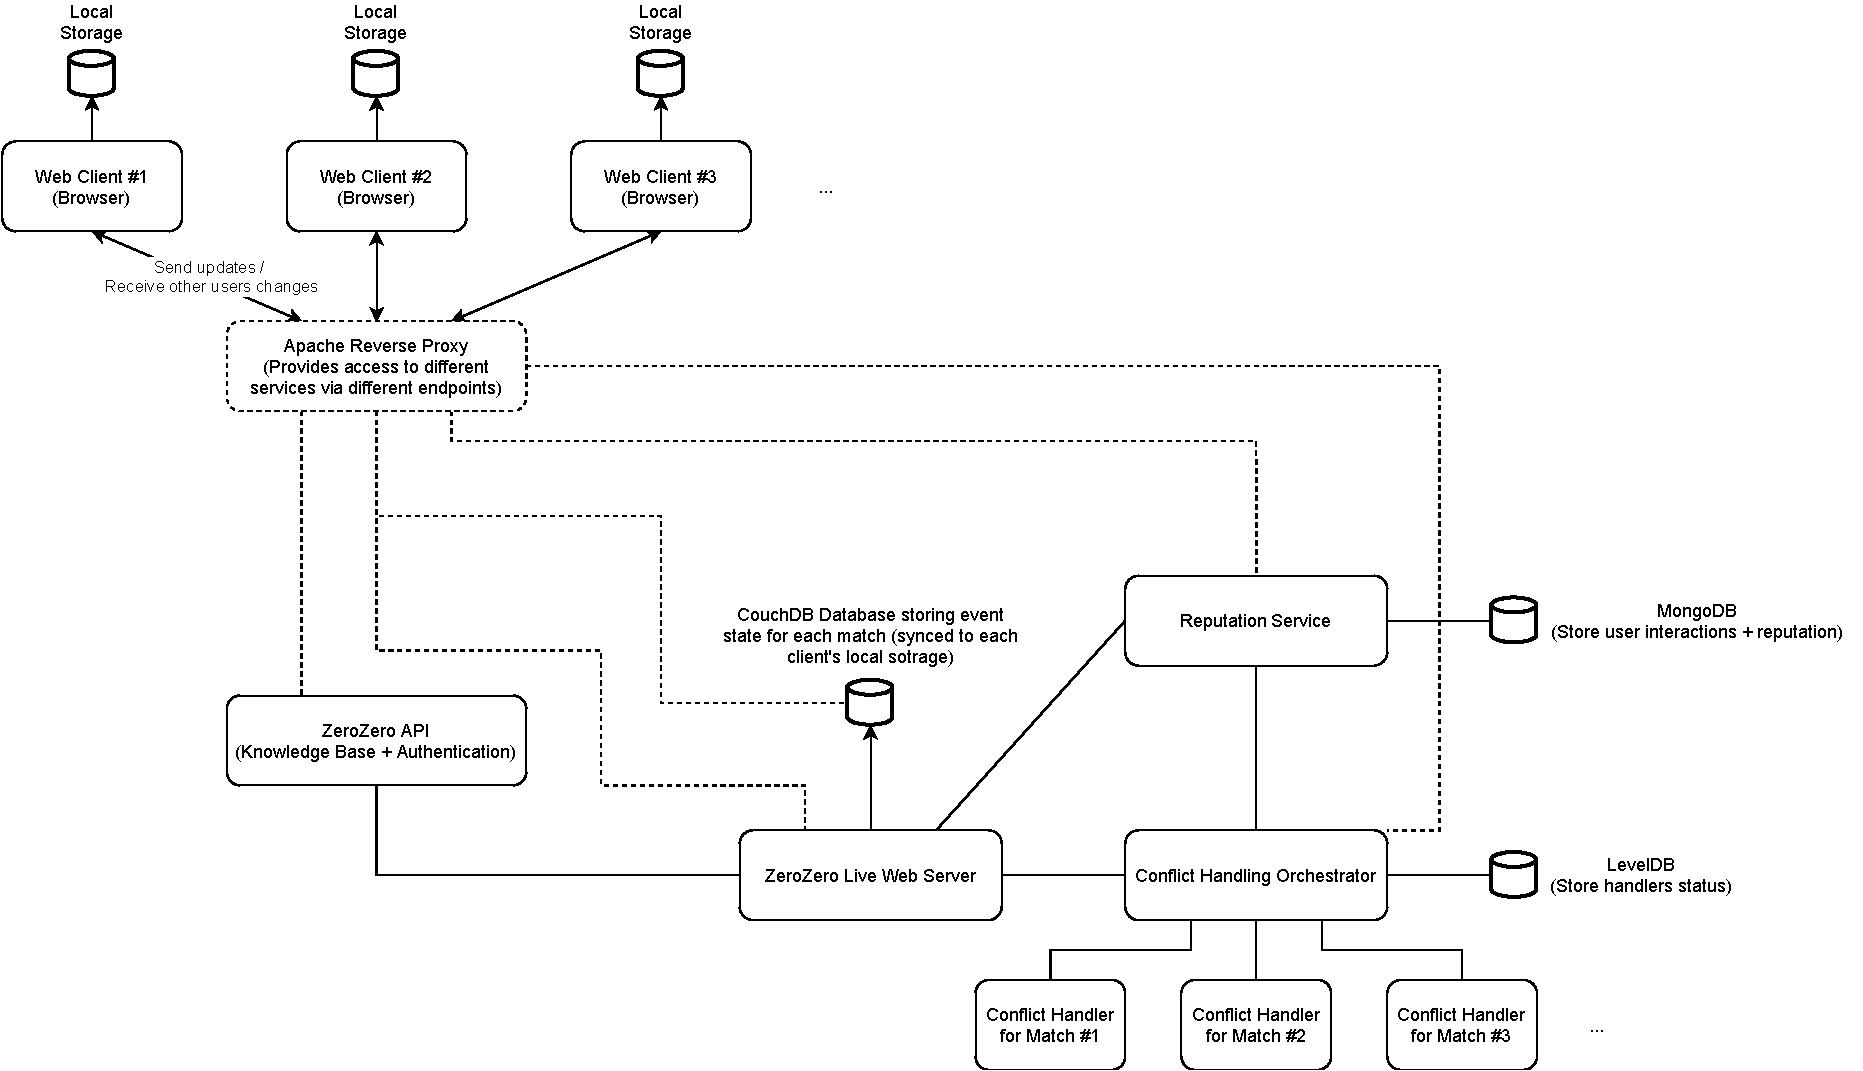
\includegraphics[width=0.9\textwidth]{zerozerolive-arch.pdf}
        \caption{High Level Architecture design of the zerozero.live system}
        \label{fig:high-level-arch}
    \end{center}
\end{figure}

\section{Offline Availability} \label{sec:prob-solution-offline-avail}
According to the research done in Chapter \ref{chap:sota}, there needs to be a way of storing state locally, in case the user is offline. Since, this application is a web application, from the alternatives presented, \textbf{localStorage} seems to be the most available among browsers\footnote{https://caniuse.com/?search=localstorage}, while fitting the project's needs. 

Currently, in the already existing \say{Proof-of-Concept}, there is an already implemented solution, which uses a local queue of requests stored in \textit{localStorage}, so as to not overwhelm the server with changes every second. This queue is \say{dumped} every 10 seconds, that is, every 10 seconds, the operations batched in the queue are sent to the server. While this allows for prevention of operations loss in case of sudden network connectivity, it might not be the best approach in terms of real-time and user experience. For example, let's say that a user generates a conflicting operation, but that operation is only sent 10 seconds later. Only then the user will see that effect on is device, when it could have happened sooner.

My proposal is to reduce the waiting time to a more reasonable 2 seconds, which, while preventing the overwhelming of messages to the server, reduces notification time and still lets the user cancel the operation before it being sent.

\section{Conflict Resolution} \label{sec:prob-solution-conflict-res}
This is a topic on which there is no clear solution. As it was seen in the research, the most well-know and used approaches are OT and CRDT. The community cannot, however, elect a clear winner\footnote{https://news.ycombinator.com/item?id=22039950}, they are just \textit{different}. On the OT side, a common approach is to use ShareDB\footnote{https://github.com/share/sharedb}, together with the JSON OT type definition\footnote{https://github.com/ottypes/json0}.

Another alternative would be to use CouchDB\footnote{https://couchdb.apache.org/} with its web browser counterpart, PouchDB\footnote{https://pouchdb.com/}. It allows for replication of state among all users, with complete control on conflict resolution: When CouchDB encounters a conflict scenario, it arbitrarily chooses a winner, deterministically, however, it keeps the conflicting version as well, which can be used to solve the conflict with custom application logic, for example, based on a reputation system, or on merging the two inputs --- Creative Resolution (Section \ref{sec:conflict-res-sota})

On the CRDT side, there are two options: Automerge\footnote{https://github.com/automerge/automerge} and GUN\footnote{https://github.com/amark/gun}. Since the latter's documentation seems to be lacking, I am removing it from the options pool. Automerge is flexible enough, allowing for server-client network architecture, as well as peer-to-peer, and it works like JSON CRDT were described to work: each user has a local copy of the JSON state, which can be locally mutated, even when offline, and it will sync automatically with other nodes. It works similarly to the CouchDB/PouchDB conflict handling, in being as much automatic as possible, but letting the application know about existing conflicts and handle them.

At this point, the ShareDB option seems to work on a lower level than the other two, and it might be unfeasible to have good results in the expected timeframe. Between CouchDB/PouchDB and Automerge, there is no clear winner, the only distinctive charateristic being that CouchDB is more mature and has been used in production for much longer. Nevertheless, the wise decision here would be to try both in a small \say{Proof-of-Concept} and further verify their usability. 

\section{Reputation System} \label{sec:problem-solution-rep-sys}
As was mentioned in the Literature Review (Section \ref{sec:rep-sys-sota}), an effective method to achieve a fair reputation system, which takes into account the time dynamics of user interactions as well as their current reputation, is to implement a personalized PageRank algorithm, which takes into account the reputation of users when calculating vouching or invalidation, in order to achieve a weighted voting system so as to provide long-term reputable users with a prize for their good behavior. Recalling the system present in \cite{Daly2009}, there are 4 rules involved in adapting the system to our use case:

\begin{enumerate}
    \item Every time a user consumes a document from an author, the author gains reputation;
    \item Every time a user consumes a document, the document gains \say{reputation} (i.e. popularity);
    \item In order to take time dynamics into account, reputation should decrease over time, so that a \say{rich-get-richer} paradigm can be avoided (both for users and for documents);
    \item Users with higher reputation matter more when calculating the document reputation changes;
\end{enumerate}

With this in mind, I propose the following rules to adapt this to our scenario:

\begin{itemize}
    \item Every time a user agrees with an input, he will improve the input's reputation according to rules 2 and 4;
    \begin{multline}
        newInputRep = oldInputRep + (1 - oldInputRep) * maxRepReward * userRep\\ * userRepInfluence
    \end{multline}
    \item Every time a user disagrees with an input (either by inputting a real-conflicting input or reporting as false/inaccurate) he will worsen the input's rep according to rules (2's reverse) and 4;
    \begin{equation}
        newInputRep = oldInputRep * (1 - maxRepPunishment * userRep * userRepInfluence)
    \end{equation}
    \item Every time a user submits a falsely-conflicting input, meaning that both users submitted the same information resulting in duplicated information, it should act as an explicit agreement with the other user's input, so it should count more, according to an $explicitAgreementBonus$ constant, which must be greater than zero to achieve the bonus effect;
    \begin{multline}
    newInputRep = oldInputRep \\+ ((1 - oldInputRep) * repReward * userRep * userRepInfluence)\\ * (1 + explicitAgreementBonus)
    \end{multline}
    \item The user gains reputation according to the average of its inputs' reputations. Only takes into account the latest inputs, referring to the last event which will trigger the reputation update;
    \begin{equation}
        newUserRep = oldUserRep + (1 - oldUserRep) * \frac{\sum inputRep}{numInputs}
    \end{equation}
    \item Each user has a reputation decay according to rule 3, the time unit should be 1 week since there's at least one relevant game per week. This prevents users that generate a lot of inputs in a single game to enjoy their reputation boost for many more games, since they need to be consistent every week: it matters more if they make an input every week than 20 inputs once every 2 or more weeks.
    This decay is on a higher level than the events, creating 20 inputs in an event is roughly the same as 1 input in an event (since the football events last around 90 minutes)
    \begin{equation}
        newUserRep = oldUserRep * decayCoefficient^{timeSinceLastUpdate}
    \end{equation}
    \item The reputation values are updated at the end of each event, according to the event's history.
\end{itemize}

\chapter{Conclusions} \label{chap:concl}


This chapter is divided into various sections. Section~\ref{sec:conc-contributions} outlines the contributions made during this work. An overview on the achieved results is present in Section~\ref{sec:conc-results}. Section~\ref{sec:difficulties} details the difficulties faced during the development and realization of this work. Finally, Section~\ref{sec:conc-future-work} will delineate future paths for this work, which can bring value to the product and research.

\section{Contributions} \label{sec:conc-contributions}

The implementation of a web application to solve the problems identified in Chapter~\ref{chap:problem} was successfully completed, resulting in a minimal production-ready product, which is, at the moment of writing, used to cover Euro2020 matches by official ZeroZero journalists. It features the real-time coverage of a match, together with the conflict resolution required to keep the data consistent. It features offline resilience, by synchronizing pending information as soon as possible. Additionally, a reputation system was developed, in order to aid the conflict resolution algorithm in case of tie. All of this was build by using a microservice architecture which was comprised of the following services:
\begin{description}
    \item[Reverse Proxy] Routes requests for the respective service, based on the requested endpoint;
    \item[ZeroZero API Proxy] A mini-proxy that routes requests for the ZeroZero API, hiding secret values such as the API Key;
    \item[Conflict Handlers Orchestrator] Manages the active handlers for each live match, and provides endpoints to start, stop and cleanup stale handlers;
    \item[Conflict Handler] Controlled by the orchestrator, listens to changes to the respective match CouchDB database, and resolves conflicts, according to the specified rules;
    \item[Reputation Service] Manages the users reputation, calculated based on the interactions during live matches on ZeroZero Live;
    \item[Web Application (Frontend)] Frontend for users to interact with the application, by allowing them to follow a match passively, or cover it by inserting events, on real-time;
    \item[CouchDB] The document database used for ZeroZero Live's events storage, allowing conflict detection and resolution;
    \item[MongoDB] The database to store user reputation information.
\end{description}

\section{Results} \label{sec:conc-results}
The research goal of this work was to study the impact of automatic conflict resolution on the user experience regarding a real-time multi-user crowdsourcing environment. Early research showed that users find that the user experience is better on environments that have automatic conflict resolution, when compared to an environment that does not have it. Research also showed that conflicts are not as common as expected, when following a game through a video stream --- TV or over the internet, not live. Nevertheless, users were content with the application and would use the application again, independently of the automatic conflict resolution feature being active or not. The fact that the application is currently being used in production validates its use case and entails a minimum level of quality and usability. Finally, it was shown that the product has two types of users, with different use cases: while the journalists require API synchronization and stability as they input a higher number of events, the casual users are more vulnerable to conflicts and rely more on an easier input experience, due to their lack of knowledge over the range of existing events.

\section{Difficulties} \label{sec:difficulties}
During the development of this project, some difficulties appeared and were tackled as best as possible. Some were solved, and others are left as future work in Section~\ref{sec:conc-future-work}. Regarding the big picture of the project, the COVID-19 pandemic meant that there were not many live matches to cover in person, which caused barriers in executing experiments with casual users. Those were mitigated by researching during TV-transmitted games, to mitigate the lack of live in-person coverages. Regarding the project itself, the synchronization with the existing ZeroZero API, in terms of storing match events was one of the hardest problems to solve, as it meant the application had two sources of truth, that must be consistent with one another at all times. Currently, that consistency is only guaranteed from ZeroZero Live to ZeroZero API --- insert, edit and delete operations on ZeroZero Live are reflected on ZeroZero --- but only insert operations on ZeroZero API will be propagated to ZeroZero Live.

\section{Future Work} \label{sec:conc-future-work}

Due to the core design of the conflict detection, some types of conflicts are not detected. Such is the case with different minute conflicts. It is very plausible for users to input the same event on consecutive minutes, but currently, since the generated documents' $\_id$s will be different, they won't conflict. This type of check must occur on insert, and the handler must check for events with the minute within a delta. If they are similar enough, or follow some to be defined criteria, they will be classified as conflicts (by re-inserting them as a document with the same id as some pivot document, regardless of the document's original minute). Regarding the reputation system, not enough tests were conducted in order to attest which is the best configuration in terms of constant values. That research would improve the system and provide insights on generic reputation systems' behavior. Finally, more tests should be done in order to fully validate the hypothesis that conflict resolution really benefits the user experience on a real-time multi-user crowdsourcing environment.


\vspace*{12mm}

%% comment next 2 commands if numbered appendices are not used
\appendix
\chapter{Services Architecture} \label{ap1:annex-high-level-arch}

This annex contains the architecture diagram of the implemented solution, representing all of its components, as explained in Chapter~\ref{chap:solution}.

\begin{landscape}
    \begin{figure}
       \centering
        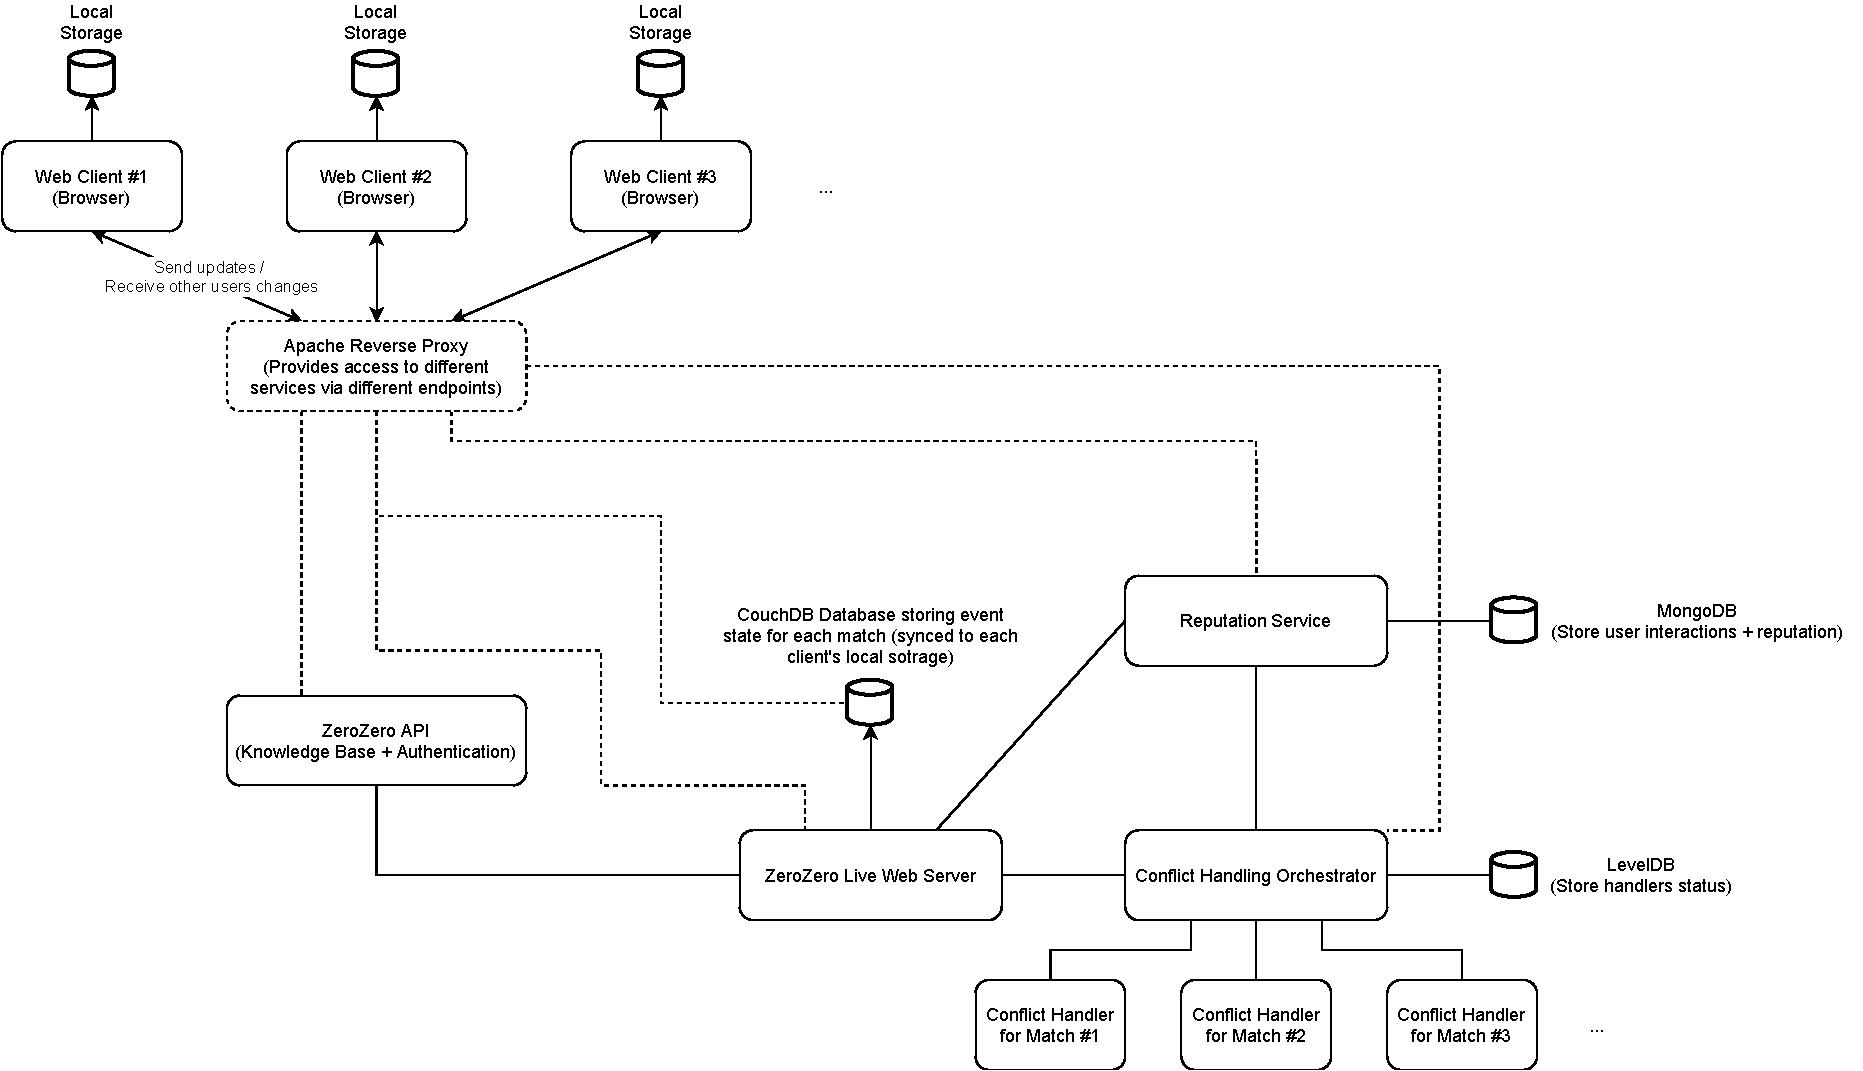
\includegraphics[height=0.9\textheight]{zerozerolive-arch.pdf}
        \caption{Services Architecture of the Application}
        \label{fig:annex-high-level-arch}
    \end{figure}
    \end{landscape}

\chapter{ZeroZero API events list} \label{annex:api-events}

\begin{longtable}{| p{.20\textwidth} | p{.60\textwidth} | p{.20\textwidth} |} 
    \caption{ZeroZero API events list (some fields were omitted for better reading purposes)} \\
    \hline
    \textbf{Event Id} & \textbf{Event Name} & \textbf{Category} \\ \hline
    \endfirsthead       
    \hline    
    \textbf{Event Id} & \textbf{Event Name} & \textbf{Category} \\ \hline       
    \endhead      
    8 & Estatísticas & 6 \\ \hline
    16 & Tempo Adicional & 6 \\ \hline
    24 & Info Jogador & 6 \\ \hline
    26 & Classificação & 6 \\ \hline
    29 & Outro Resultado & 6 \\ \hline
    43 & Lance polémico & 6 \\ \hline
    52 & VAR & 6 \\ \hline
    64 & Estatísticas Jogo & 6 \\ \hline
    78 & Fora de jogo & 6 \\ \hline
    79 & Castigado & 6 \\ \hline
    80 & Árbitros & 6 \\ \hline
    81 & Apresentação VAR & 6 \\ \hline
    83 & Canto & 6 \\ \hline
    3 & Comentário & 5 \\ \hline
    19 & Informação & 5 \\ \hline
    20 & Lesão grave & 5 \\ \hline
    22 & Homem do Jogo & 5 \\ \hline
    31 & Informação R. & 5 \\ \hline
    32 & Onzes Definidos & 5 \\ \hline
    36 & Info Pré-Jogo & 5 \\ \hline
    42 & Opinião & 5 \\ \hline
    46 & Antevisão & 5 \\ \hline
    47 & Rescaldo & 5 \\ \hline
    49 & Atualização de Resultado & 5 \\ \hline
    50 & Suplentes & 5 \\ \hline
    54 & Espetadores & 5 \\ \hline
    55 & Lesão & 5 \\ \hline
    5 & Substituição & 4 \\ \hline
    9 & Apito Inicial & 3 \\ \hline
    10 & Fim 1ª Parte & 3 \\ \hline
    11 & Início 2ª Parte & 3 \\ \hline
    12 & Fim 2ª Parte & 3 \\ \hline
    13 & Apito Final & 3 \\ \hline
    14 & Início Prolong. & 3 \\ \hline
    15 & Fim Prolong. & 3 \\ \hline
    56 & Fim 1ª Parte Prolongamento & 3 \\ \hline
    57 & Início 2ª Parte Prolongamento & 3 \\ \hline
    2 & Cartão Amarelo & 2 \\ \hline
    4 & Cartão Vermelho & 2 \\ \hline
    1 & Golo & 1 \\ \hline
    6 & Oportunidade Grande & 1 \\ \hline
    7 & Auto-Golo & 1 \\ \hline
    17 & Penalti Marcado & 1 \\ \hline
    18 & Penalti Falhado & 1 \\ \hline
    23 & Penalti Assin. & 1 \\ \hline
    35 & Penálti falhado & 1 \\ \hline
    44 & Golo invalidado & 1 \\ \hline
    53 & Oportunidade Pequena & 1 \\ \hline
    67 & Bola à barra & 1 \\ \hline
    68 & Bola ao poste & 1 \\ \hline
    84 & Assistência & 1 \\ \hline
    25 & Estatisticas 11 & 0 \\ \hline
    27 & Estatísticas Nac & 0 \\ \hline
    28 & Vídeo & 0 \\ \hline
    30 & Fotos & 0 \\ \hline
    34 & Penálti marcado & 0 \\ \hline
    37 & Info Pós-Jogo & 0 \\ \hline
    38 & JOG - Golos na Seleção (Único) & 0 \\ \hline
    39 & EQ - Resultados & 0 \\ \hline
    41 & Sondagem & 0 \\ \hline
    45 & Curiosidade PM & 0 \\ \hline
    48 & Fim de Relato & 0 \\ \hline
    51 & Bola ao ferro & 0 \\ \hline
    58 & Opinião com Foto & 0 \\ \hline
    60 & 5.ª falta & 0 \\ \hline
    61 & Time-out & 0 \\ \hline
    62 & Livre 10m assinalado & 0 \\ \hline
    63 & Cincos definidos & 0 \\ \hline
    65 & 5x4+GR & 0 \\ \hline
    66 & Faltas (Futsal) & 0 \\ \hline
    69 & Livre 10m Falhado & 0 \\ \hline
    70 & Livre 10m marcado & 0 \\ \hline
    71 & Livre direto assinalado & 0 \\ \hline 
    72 & Livre direto marcado & 0 \\ \hline
    73 & Livre direto falhado & 0 \\ \hline
    74 & 10.ª falta & 0 \\ \hline
    75 & 15.ª falta & 0 \\ \hline
    76 & 20.ª falta & 0 \\ \hline
    77 & Cartão Azul & 0 \\ \hline
    % \label{tab:myfirstlongtable}
\end{longtable}

% \begin{figure}[h]
%     \centering
%     \rotatebox{90}{
%         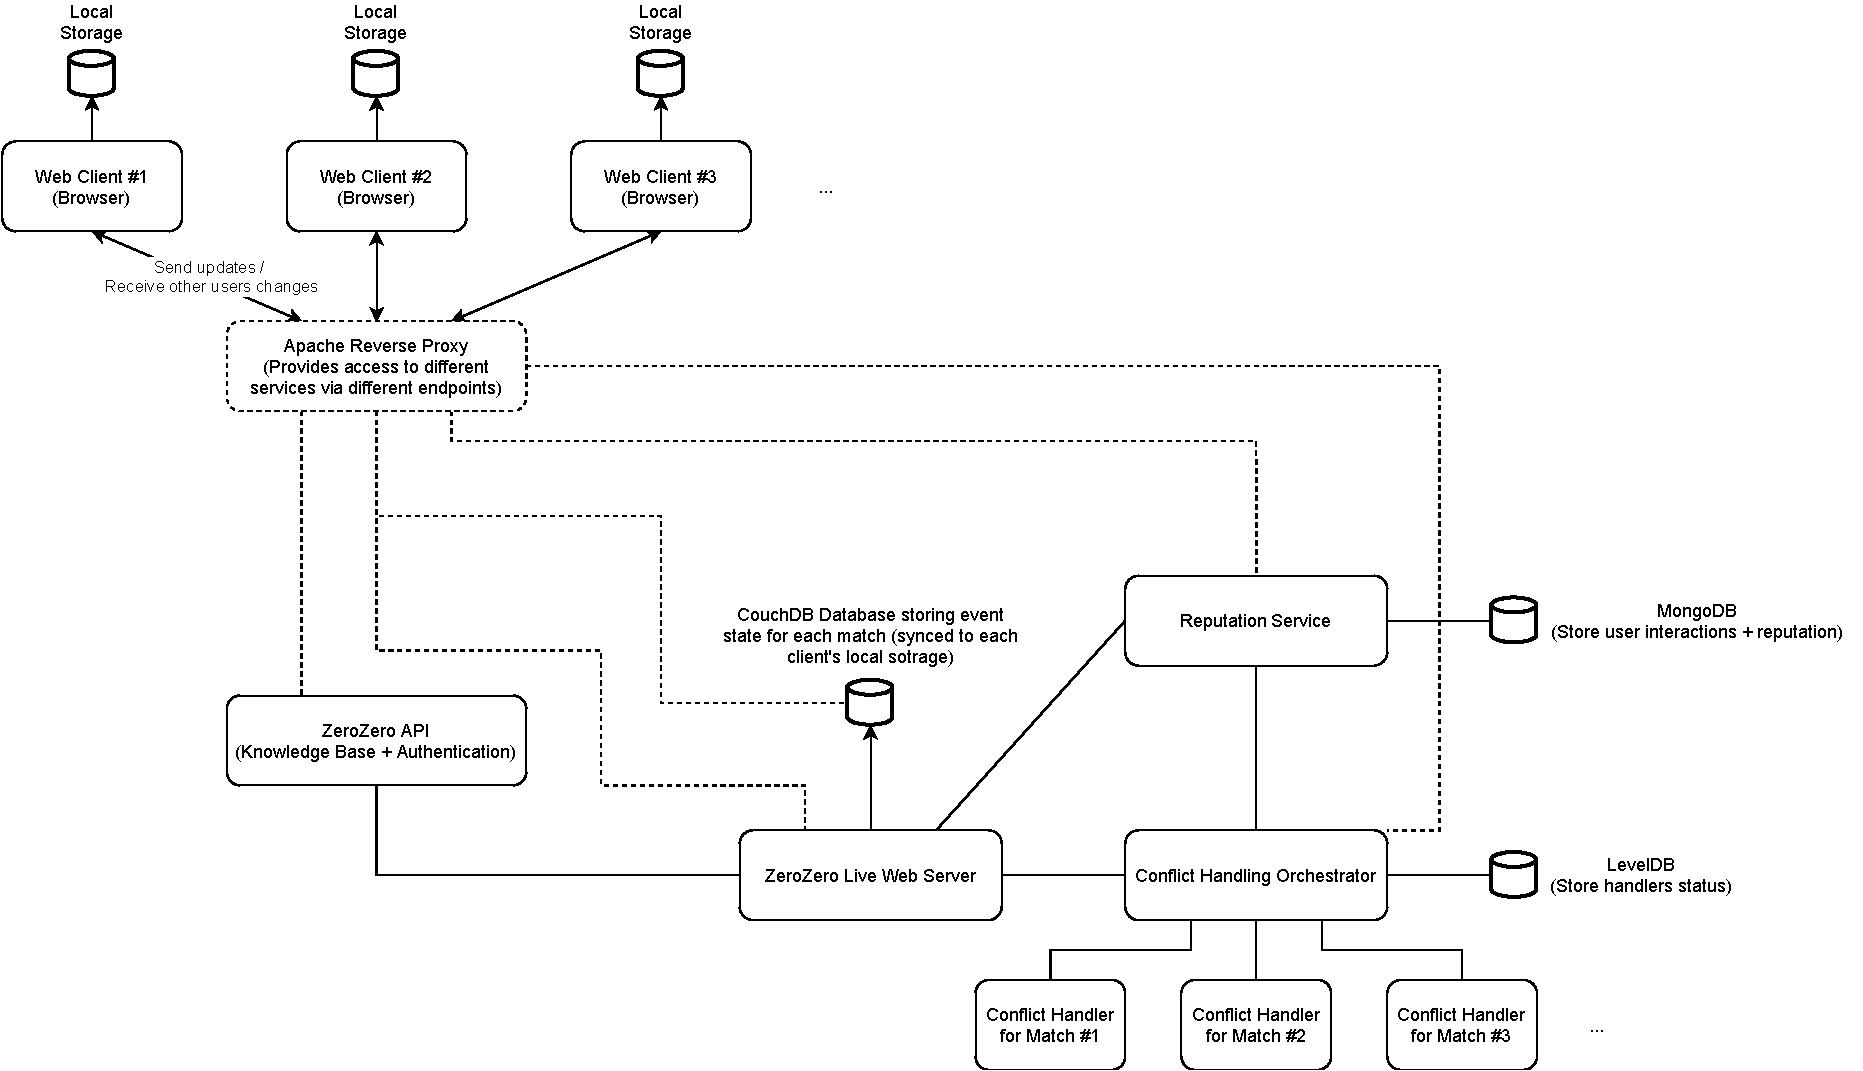
\includegraphics[width=0.5\textheight]{zerozerolive-arch.pdf}
%         % \caption{Services Architecture of the Application}
%     }

%     \end{figure}
    



%%----------------------------------------
%% Final materials
%%----------------------------------------

%% Bibliography
%% Comment the next command if BibTeX file not used
%% bibliography is in ``myrefs.bib''
\PrintBib{myrefs}

%% Index
%% Uncomment next command if index is required
%% don't forget to run ``makeindex thesis'' command
%\PrintIndex

\end{document}
